\documentclass[crop,tikz,border=1px]{standalone}

\usetikzlibrary{arrows,positioning,scopes,automata,calc}

\begin{document}
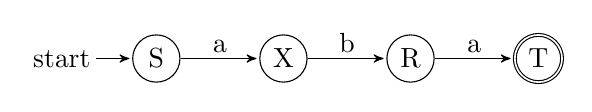
\begin{tikzpicture}[->,>=stealth',shorten >=1pt,auto,node
  distance=1cm,inner sep=2pt,
  mystate/.style={state,text centered,minimum size=.6cm}]

  \node[initial,mystate] (q0) {S};
  \node[mystate] (q1) [right=of q0] {X};
  \node[mystate] (q2) [right=of q1] {R};
  \node[accepting,mystate] (q3) [right=of q2] {T};

  \draw (q0) edge node {a} (q1)
        (q1) edge node {b} (q2)
        (q2) edge node {a} (q3);

\end{tikzpicture}
\end{document}
